\documentclass[../main.tex]{subfiles}
\begin{document}


\section{Data Visualisation: A Brief History}\label{brief-history}

Data visualisation, which can be thought of as the practice of
representing information in a visual modality \cite{hinterberger_2009},
is difficult to concretely define, classify, and categorise. For most of
us, vision is the primary medium through which we interact with the
world around us; in this way, data visualisation may be thought of as an
extension of art and the written word. Both art and writing are ancient
phenomena, with evidence for the former being found in the prehistoric
period some 66,000 years ago \cite{standish_2025}, and evidence for the
latter emerging as Mesopotamian cuneiform around 3200 B.C.E
\cite{schmandt_2014}. Broadly, the literature indicates that art emerged
prior to the written word; this speaks volumes of the human instinct to
represent our thoughts, feelings, emotions, and the ways that we
interact with the world pictorially. This instinct has not waned, and
modern computing makes it easier than ever for those with no technical
or artistic skills to create graphics and visualisations that \emph{tell
stories} about our data in ways which are both beautiful and
informative.

When, then, should we consider to be the emergence of data visualisation
as a human practice? Schmandt-Besserat
\cite{schmandt_1978, schmandt_2014} considers clay counting tokens to be
the direct precursor of the written word; while the evidence for this
link is controversial \cite{robson_2007}, the existence of such tokens
is not. With each shape of token representing a certain amount of a
certain good (measures of grain, jars of oil, etc.), this system could
be considered a very early, simple form of data visualisation (or
physicalisation, see Jansen et al., 2015 \cite{jansen_2015}). Similarly,
there is limited evidence of prehistoric cartographic drawings
\cite{muhly_1978}, which may also be considered a form of, or related
to, data visualisation. While I am not asserting that data visualisation
is older than writing, or that ancient map drawings are equivalent to
modern graphics, the existence of these representations emphasises the
convenience that symbols and signs represent for humans; making sense of
our world and the relationships therein is often easier through pictures
as opposed to only words and/or numbers, a principle which I consider
key for this thesis.

Moving on, then, to the kind of pictorial representation that modern-day
students and scientists would firmly recognise as ``data
visualisation''. Tufte and Graves-Morris, in 1983's seminal \emph{The
Visual Display of Quantitative Information} \cite{tufte_1983}, describe
an unattributed time series illustration from the 10th or 11th century,
itself described by Funkhouser in 1936 \cite{funkhouser_1936} as being
discovered by Sigmund Günther in 1877. This illustration is included
here in Figure~\ref{fig-early-time-series}.

\begin{figure}

\centering{

\includegraphics[width=\textwidth]{../supplied_graphics/tufte_1983.png}

}

\caption{\label{fig-early-time-series}Reproduced in Tufte and
Graves-Morris, 1983 \cite{tufte_1983} from Funkhouser, 1936
\cite{funkhouser_1936}.}

\end{figure}%

This illustration purports to show the movements of planetary bodies as
a function of time, although Funkhouser considered it little more than a
``schematic diagram\ldots for illustrative purposes''
\cite{funkhouser_1936}. Regardless, the recognisable grid lines and
sinusoidal variation in the curves are ideas that would not appear again
for another 600-700 years, after which they would become mainstream
visualisation techniques. In the mid-14th century, French philosopher
Nicole Oresme demonstrated an understanding of graphing by plotting
proto-bar charts, and by the 16th century, advances in cartography,
photography, and mathematics laid the ground for an explosion in data
visualisation.

The 17th century saw the birth of geometry and coordinate systems, error
measurement, probability, and demographic statistics. With these
scientific advancements came the advancements in data visualisation
needed to communicate these concepts. For example, in 1626, Scheiner
used what Tufte would later term the ``principle of small multiples''
\cite{tufte_1983} to illustrate how configurations of sunspots change
over time (see Figure~\ref{fig-sunspots}).

\begin{figure}

\centering{

\includegraphics[width=\textwidth]{../supplied_graphics/sunspots.png}

}

\caption{\label{fig-sunspots}Scheiner's (1626) plot detailing how
configurations of sunspots change over time. This technique would later
be referred to as the ``principle of small multiples'' by Tufte.}

\end{figure}%

\begin{figure}

\centering{

\includegraphics[width=\textwidth]{../supplied_graphics/snow_cholera.jpg}

}

\caption{\label{fig-cholera}John Snow's (1854) map of cholera cases in
Soho, London. Using this data visualisation, Snow was able to
demonstrate a link between cholera cases and a contaminated water
supply.}

\end{figure}%

\begin{figure}

\centering{

\includegraphics[width=\textwidth]{../supplied_graphics/minard_napoleon.jpg}

}

\caption{\label{fig-napoleon}Charles Joseph Minard's (1869) flow diagram
of Napoleon's botched invasion of Russia in 1812-1813. This diagram
shows Napoleon's advance and retreat on Moscow. The width of the orange
and black columns encodes the size of the Grande Armée. The temperature
scale on the lower portion of the graph illustrates the weather
conditions during the retreat, with a freezing Russian winter causing
high rates of attrition.}

\end{figure}%

\begin{figure}

\centering{

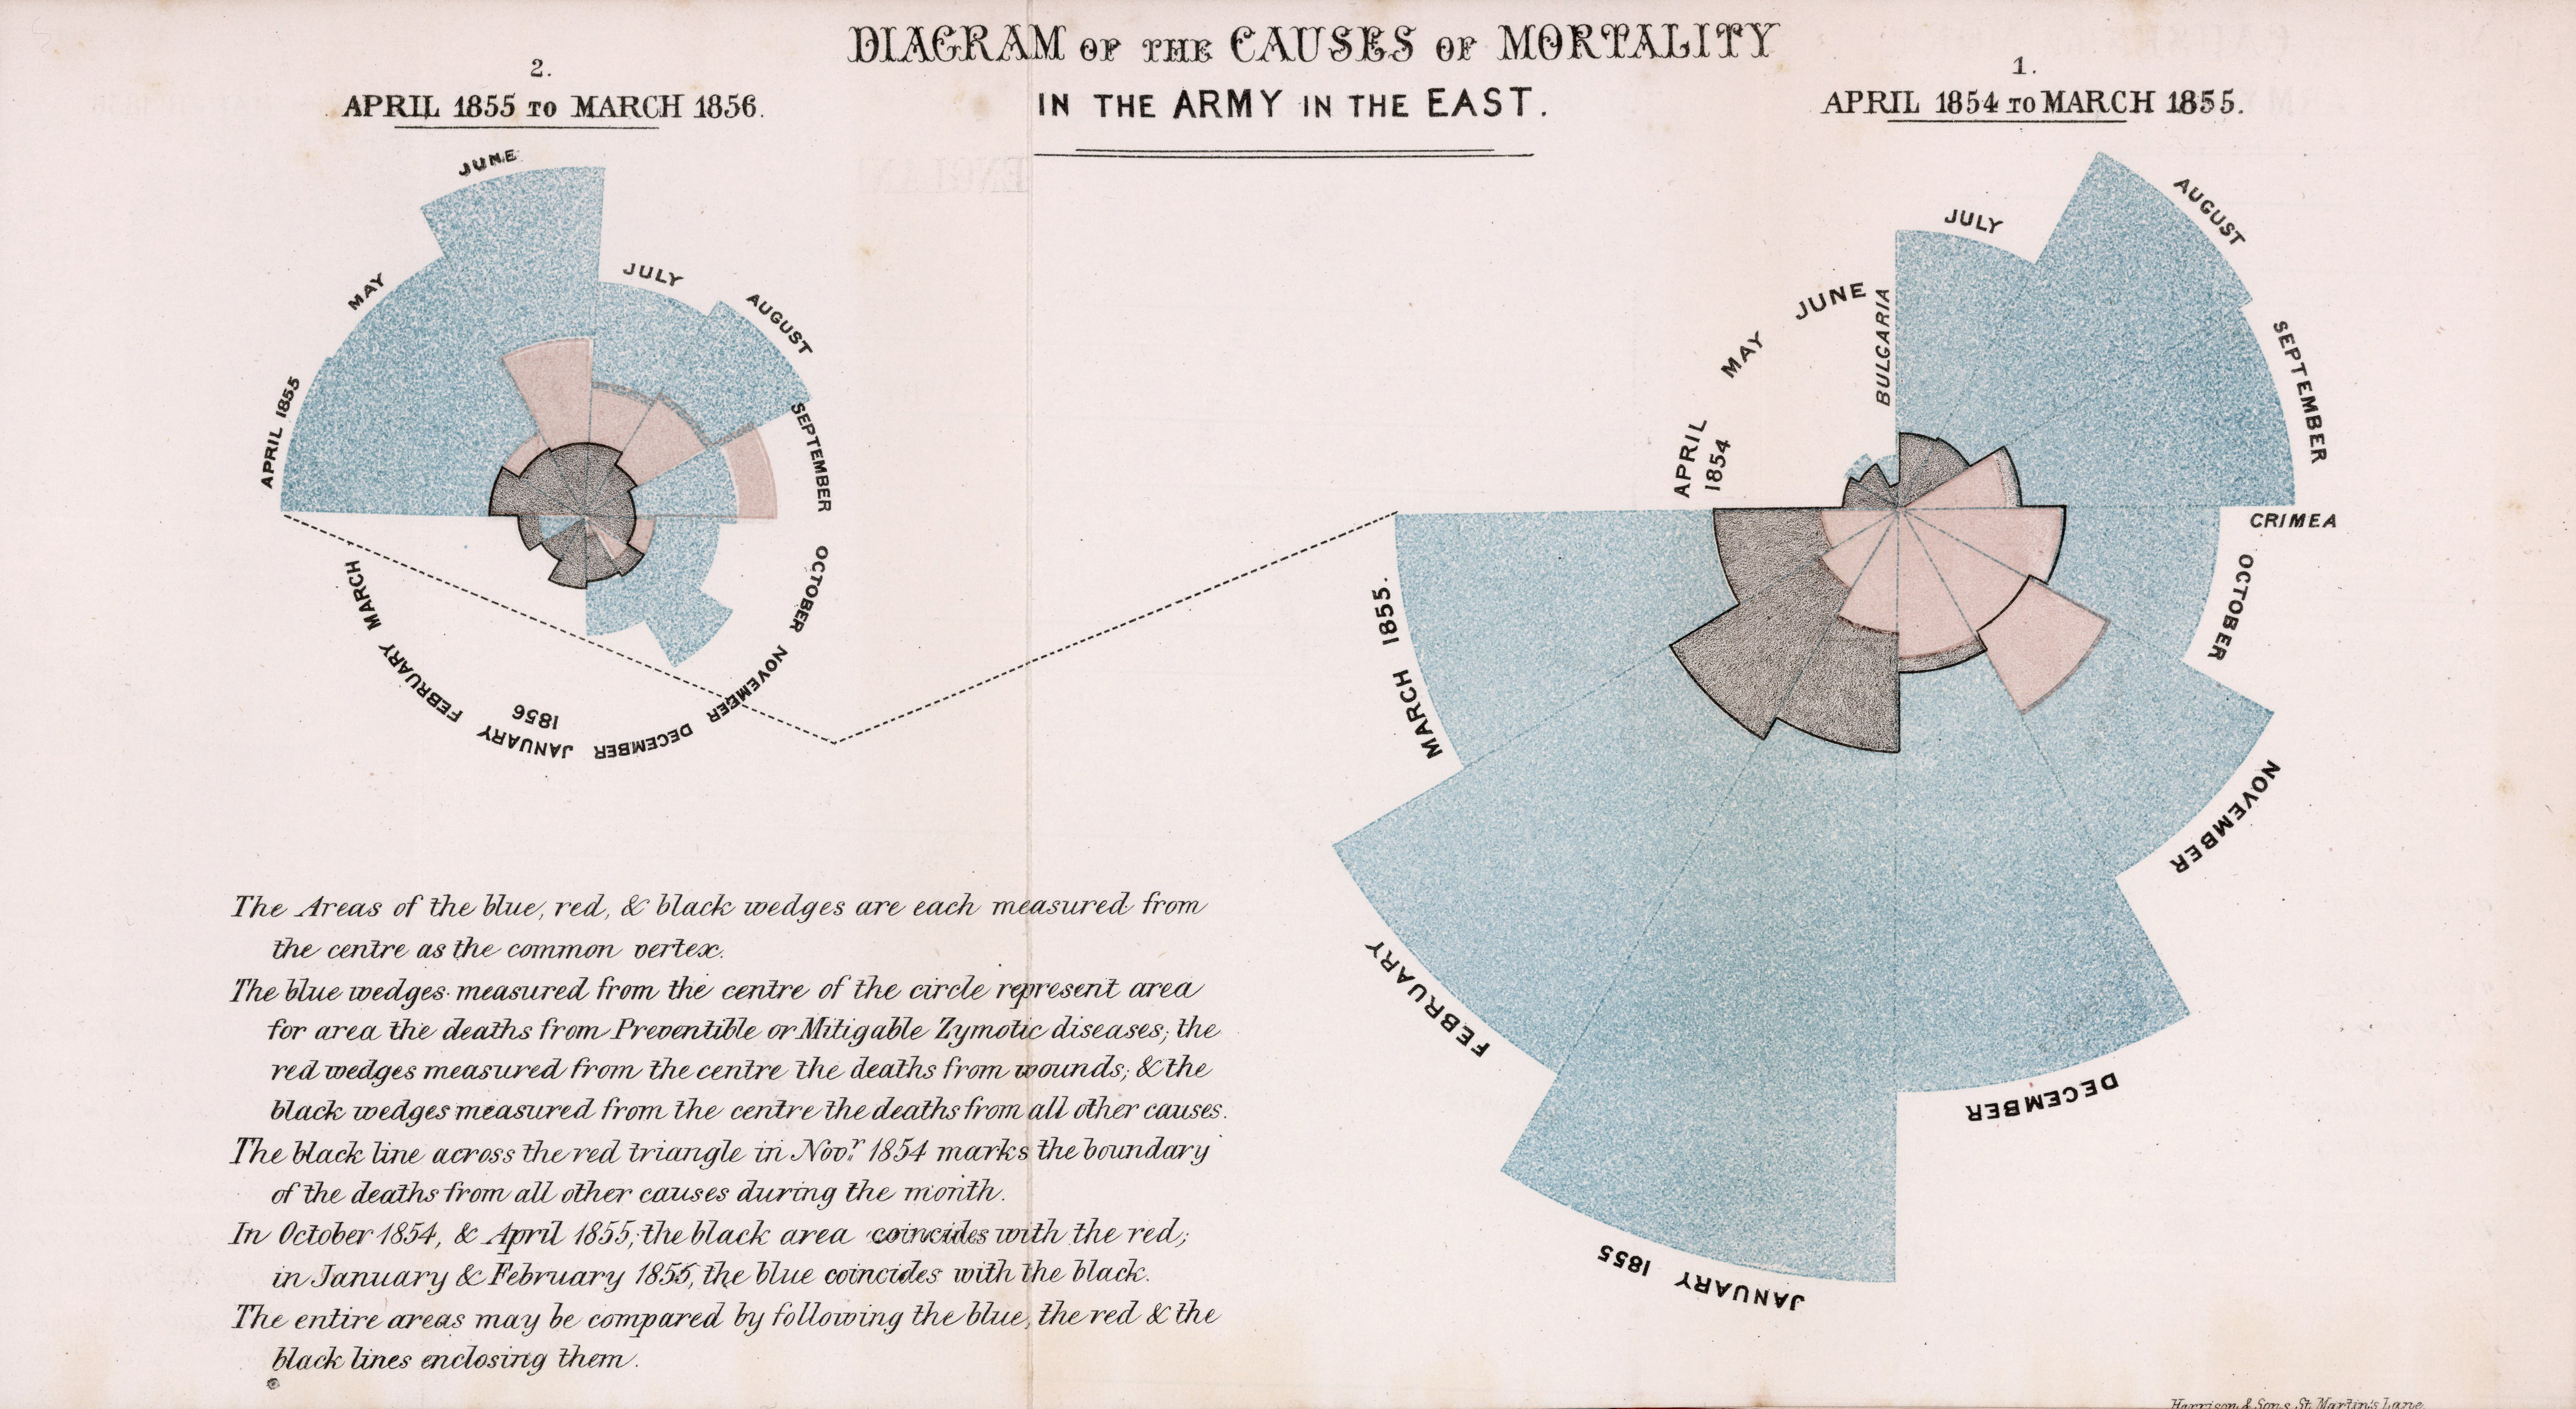
\includegraphics[width=\textwidth]{../supplied_graphics/nightingale-rose.jpg}

}

\caption{\label{fig-nightingale}Florence Nightingale's (1858) polar area
chart illustrates the causes for mortality among British soldiers during
the Crimean War. Data visualisations of this type were used to
illustrate that in reality, more British soldiers died from preventable
disease than were killed by the enemy, and were used as part of a
campaign to improve sanitation on the front lines.}

\end{figure}%

The latter half of the 19th century, the so-called ``Golden Age of
Statistical Graphics'' \cite{friendly_2008} saw the rise of forms of
data visualisation that begin to look remarkably similar to the graphs
and informatics seen in mass media and scientific publication today. The
most notable examples of these are John Snow's cholera map, which was
able to link the incidence of cholera to a contaminated water pump in
London (Figure~\ref{fig-cholera}), Charles Joseph Minard's flow chart of
the Napoleonic invasion of Russia (Figure~\ref{fig-napoleon}), and
Florence Nightingale's rose diagrams (polar area charts in the modern
parlance, see Figure~\ref{fig-nightingale}). In each of these graphs,
visualisation is used with different intent. In John Snow's cholera map,
visualisation was used to track cases of a deadly disease, and
facilitated a novel linkage between cholera and contaminated drinking
water. In Charles Joseph Minard's flow chart of Napoleon's failed 1812
invasion of Russia, a total of six variables are displayed to tell the
data story, allowing the viewer to appreciate the movements of the
Grande Armée, its diminishing size owing to attrition, and the freezing
temperatures that largely caused that attrition. Florence Nightingale's
polar area chart depicts the causes of mortality amongst British troops
in the Crimean War; charts such as this were used to successfully
campaign for better sanitation in hospitals and on the front lines.

In all of these visualisations, data was used to accentuate
storytelling. In some cases, this lead to critical discoveries that
saved lives, and in others, it simply facilitated a greater
understanding and appreciation of the data. In either case,
visualisation is used effectively to appeal to our affinity for visual
storytelling. An appetite for precision defined the approach to
statistical thinking, and by extension, data visualisation, in the first
half of the 20th century. Statistical graphics finally became
mainstream, and were implemented in curricula and used in government,
commerce, and finance. This period also marks the beginning of graphical
methods being used to generate new scientific insights, a trend which
would only accelerate throughout the next century.

Significant developments in the latter half of the 20th century laid the
final brick in the foundations of what would become the modern data
visualisation landscape. John W. Tukey's \emph{The Future of Data
Analysis} \cite{tukey_1962} proposed a separation between data analysis
and mathematical statistics. This work would become hugely influential,
and Tukey would go on to invent a great number of analysis-driven data
visualisations, including stem-leaf plots and box plots, both of which
are now commonplace in software packages and statistics education. In
1967, Jacques Bertin \cite{bertin_1967} published \emph{Sémiologie
graphique} (\emph{Semiology of Graphics}), organising the perceptual
elements of data visualisations according to their features and their
relationships to the underlying data; this work would be influential for
Leland Wilkinson's \emph{Grammar of Graphics} \cite{wilkinson_1999},
which in turn influenced the \texttt{ggplot2} package
\cite{wickham_2016} that is used extensively in this thesis.

\begin{figure}

\centering{

\includegraphics[width=\textwidth]{../supplied_graphics/rug_density.png}

}

\caption{\label{fig-rug-density}Major milestones in the development of
data visualisation illustrated using a rug plot and density estimate.
This figure is taken from Friendly (2008) \cite{friendly_2008}.}

\end{figure}%

Since then, both the practice and study of data visualisation have
become thoroughly mainstream. Students are taught to visualise data
early on, and the propagation of both software and powerful computing
hardware have brought advanced techniques, such as high dimensional
visualisation and massive datasets, into the home. To summarise the
timeline of developments in data visualisation over the last 500 years,
I include a rug and density plot from Friendly (2008)
\cite{friendly_2008} in Figure~\ref{fig-rug-density}. Recounting a full
and detailed history of the practice and study of data visualisation
would require much more than a single thesis, and has been done to a
very high standard elsewhere \cite{friendly_2008, friendly_2021}. Given
that this thesis is focused on the perception of correlation in
scatterplots, the remainder of the chapter is primarily limited to
discussions of relatedness, correlation, and scatterplot visualisations.

\section{Relatedness \& Correlation}\label{relatedness-and-correlation}

In Experiment 5, correlation was operationalised as \emph{Strength of
Relatedness}. To make my research accessible, I start from here; two (or
more) things are related if a change in one is associated with a change
in the other(s). In reality, however, the data visualisation under
investigation, scatterplots, do not visualise relatedness, but
correlation. Correlation refers to a specific statistical relationship,
which I explore from first principles below.

Francis Galton was the first to formally introduce the concept of
\emph{co-relation} in 1888 \cite{galton_1888}. He derived a definition
of correlation as a by-product of his invention of statistical
regression, first describing this new property by way of anthropometric
data relating to the measurement of different parts of the body. Early
in this brief, but significant, paper, Galton puts forward a basic
definition of correlation:

\begin{quotation}
  ``Two variable organs [of the body] are said to be co-related when the variation of the one is accompanied on the average by more or less variation of the other, and in the same direction.''
\end{quotation}

Measuring a variety of anatomical distances, including head lengths and
heights of a range of ``not wholly fully-grown'' males, Galton first
provides medians and semi-interquartile ranges as a measure of error.
Plotting the semi-interquartile ranges (Q-units) of two variables
against each other and calculating the slope of the line allowed Galton
to devise a new, unitless measure of co-relatedness, which he termed r.
This has since been lauded as a prime example of a mathematical
discovery made based on observed data. This method is imprecise, as it
requires intuition of a line-of-best-fit based on a hand drawn plot, but
is credited as the first full conceptual definition of a measure of
correlation; it should be noted that there was no concept of negative
correlation at this point. Galton's work did not take place in
isolation, and the preceding 60 years featured famous names, such as
Gauss and Darwin, skirting around the idea of correlation without
recognising its importance; Lee Rodgers \& Nicewander (1988)
\cite{lee_1988} provide an excellent overview of this period.

Building on Galton's groundbreaking work, his younger, more
mathematically-minded student, Karl Pearson, developed the Pearson
Product-Moment correlation (Pearson's \emph{r}) in 1895 \cite{lee_1988}
based on initial formulae by Bravais (1844) \cite{bravais_1844}. This
measure has been remarkably persistent, remaining unchanged for well
over a century. In fact, many other measures of correlation, such as
Spearman's \(\rho\), the point-biserial correlation, and the \(\phi\)
coefficient are actually special cases of Pearson's \emph{r} applied to
different types of data \cite{henrysson_1971}; such is the dominance of
the measure. Equation 2.1 defines Pearson's \emph{r}:

\begin{equation}
  r = \frac{\sum_{i=1}^{n} (x_i - \bar{x})(y_i - \bar{y})}{\sqrt{\sum_{i=1}^{n} (x_i - \bar{x})^2 \sum_{i=1}^{n} (y_i - \bar{y})^2}}
\end{equation}

In this equation, \(\bar{x}\) and \(\bar{y}\) are the means of each
variable. \(x_i\) and \(y_i\) are the individual values of each variable
in question. In the numerator, the sum of the products of the difference
between each value of \(x\) and \(y\) and their means are found; this
value represents the degree of deviation of all points from the
regression line. Then, in the denominator, this value is divided by the
magnitude of the sum of the product of said deviations; squaring and
finding the square root of these values provides the unsigned magnitude.
In statistical language, Pearson's \emph{r} finds the covariance of two
variables, then divides this value by the product of both variables'
standard deviations. Completing this calculation provides a measure of
the overall distance between the observed values and a fitted least
squares regression line, and provides a single value of \emph{r} that
describes how strongly related two variables are.

\section{Visualising Correlation}\label{visualising-correlation}

\begin{figure}

\centering{

\includegraphics[width=\textwidth]{2_related_work_files/figure-latex/fig-anscombe-1.pdf}

}

\caption{\label{fig-anscombe}Anscombe's quartet \cite{anscombe_1973}.
Each scatterplot depicts datasets with identical means (\(x\) = 9, \(y\)
= 7.5), regression coefficients (\(y\) on \(x\) = 0.5), standard errors
(0.118), and Pearson's \emph{r} values (≈ 0.816).}

\end{figure}%

Of course, while mathematically sound, a single value provides no
information about the distribution of variables from which it was
derived. To do this, the data must be examined visually. Here arises a
parallel; in much the same way as Francis Galton used a
proto-scatterplot to formulate his definition of correlation, so must
data visualisation be used to tell the story behind a value of Pearson's
\emph{r}. The need for visualisation is most viscerally illustrated by
Anscombe's quartet \cite{anscombe_1973}, which is recreated in
Figure~\ref{fig-anscombe} using a dataset from the \texttt{datasets}
core package \cite{r_core} in R. Anscombe's quartet \cite{anscombe_1973}
describes four simple datasets that are identical with regards to a
range of statistical measures. They feature the same number of
observations, the same means, regression coefficients, regression line
equations, sums of squares, estimated standard errors, and correlation
coefficients. A simple examination of these statistics would lead to the
conclusion that the datasets are identical; in reality, there are
significant differences between them that can only be seen via
visualisation.

In this thesis, the primary concern is correlation and the ways in which
people interpret it from scatterplots. The remainder of this section
examines the history and current landscape of correlation
visualisations. Starting with Galton's scatterplot precursors, I then go
on to discuss the development of the familiar modern scatterplot through
the examination of a number of impressive use cases. Following that, I
review the current landscape of correlation visualisation, including the
more recent use of other, non-scatterplot graphs.

\subsection{History}\label{history-corr-viz}

\begin{figure}

\centering{

\includegraphics[width=\textwidth]{2_related_work_files/figure-latex/fig-galton-hand-plot-1.pdf}

}

\caption{\label{fig-galton-hand-plot}Francis Galton's original plot
comparing the semi-interquartile ranges of stature (height) and cubit
(forearm length). The plot has been recreated using \texttt{ggplot2} on
the right.}

\end{figure}%

As mentioned in Section \ref{relatedness-and-correlation}, Francis
Galton based his initial formulation of the correlation coefficient on
hand-drawn plots of the semi-interquartile ranges of two variables.
Figure~\ref{fig-galton-hand-plot} contains a negative scan of Galton's
original plot, along with a modern recreation using \texttt{ggplot2}.
Despite the importance of graphics like these for Galton's discovery of
regression, statistical correlation, and the relationship between these
and the bivariate density function \cite{friendly_2005}, an earlier
example of a scatterplot can be found in work on the orbits of twin
stars by John F. W. Herschel \cite{herschel_1833}. Unfortunately, this
scatterplot was never printed in Herschel's 1833 manuscript, however it
can be inferred thanks to a detailed description of both the figure and
the logic behind it. In short, Herschel wished to ascertain the orbits
of binary star systems by using (often imprecise) astronomical
measurements of certain angles and distances made over a long period of
time. It is the imprecision in measurement which necessitated data
visualisation, as precise measurements would allow common astronomical
principles to provide precise solutions. First specifying the axes,
angle of position (\(y\)) and date of observation (\(x\)), and grid
lines, Herschel then describes plotting points and drawing, by hand, a
line-of-best-fit. A particularly enlightening quote
\cite{herschel_1833}, with original emphasis, is reproduced below:

\begin{quotation}
    ``Our next step, then, must be to draw, by the mere judgement of the eye, and with
a free but careful hand, not \textit{through}, but \textit{among} them, a curve presenting as few
and slight departures from them as possible, consistently with this character of 
large and graceful sinuosity, which must be preserved at all hazards...''
\end{quotation}

From this smoothed-by-eye line, Herschel was able to calculate the
parameters that determined the rotation of the \(\gamma\)Virginis
system. Herschel beat out Galton by more than 50 years to claim the
first scatterplot, in a remarkable feat of using graphing to solve an
astronomical problem. Just a few decades after Galton had discovered the
concept of correlation, yet another astronomical example of a
scatterplot can be found in the Hertzsprung-Russell diagram, created
independently by both Ejnar Hertzprung and Henry Norris Russell in
1911-1913 \cite{montmerle_2011}. This type of scatterplot, which still
sees use in modern astronomy, plots stellar luminosity against colour
(temperature). I have plotted an HR diagram in Figure~\ref{fig-HR-plot}
using the HYG database \footnote{https://www.astronexus.com/projects/hyg}.

\begin{figure}

\centering{

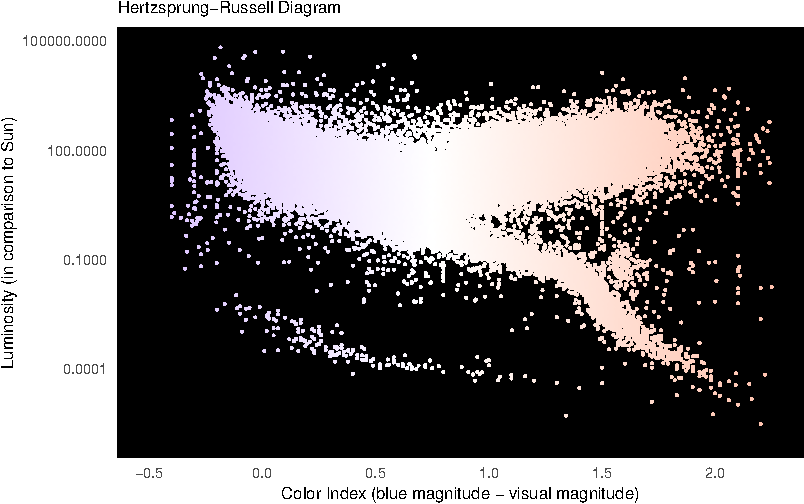
\includegraphics[width=\textwidth]{2_related_work_files/figure-latex/fig-HR-plot-1.pdf}

}

\caption{\label{fig-HR-plot}Hertzsprung-Russell diagram of colour index
against stellar luminosity. The code for this plot was taken from John
Russell's (no relation) blog \cite{russell_2025}.}

\end{figure}%

The clear band that can be seen in Figure~\ref{fig-HR-plot} from
top-left to bottom right are ``main sequence'' stars. It was only by
visualisation that astronomers were able to determine that there were
laws that govern the formation and evolution of stars. Spence and
Garrison \cite{spence_1993} conducted a detailed analysis of the history
and development of HR diagrams, and conclude that they represent a
``shining example of the power of graphic display''. Again, it was the
ability of the data visualisation to facilitate pattern recognition in
its human viewers that was so crucial to its success.

While this section has not been an exhaustive list of every scatterplot
and scatterplot-related plot that has prominently featured in scientific
publishing since Herschel's initial description and Galton's initial
formulation of correlation, I hope that I have conveyed the importance
of this visualisation type. As we will see in Section
\ref{present-landscape-corr-viz}, the landscape of correlation
visualisation is now much broader, however the humble scatterplot still
remains a crucial part of the visualiser's toolbox. From its origins as
a way of inferring astronomical relationships, to its use in the
discovery of correlation, the standard scatterplot remains largely
unchanged to this day; this thesis charts the development of a new type
of scatterplot that draws on key elements of human perception to
increase its utility in correlation visualisation, however it is
important to pay homage to the history of the visualisation as a
valuable tool for those willing and able to use graphing to solve
scientific problems.

\subsection{Present Landscape}\label{present-landscape-corr-viz}

\begin{figure}

\centering{

\includegraphics[width=\textwidth]{2_related_work_files/figure-latex/fig-other-corr-viz-1.pdf}

}

\caption{\label{fig-other-corr-viz}From top-left to bottom-right:
Parallel Coordinates Plot (PCP) built with the \texttt{GGally} package
\cite{ggally}; Stacked area plot; radial stacked bar plot (doughnut
plot); radar plot. Each plot uses the same dataset with an \emph{r}
value of 0.6.}

\end{figure}%

\begin{figure}

\centering{

\includegraphics[width=\textwidth]{2_related_work_files/figure-latex/fig-remixes-1.pdf}

}

\caption{\label{fig-remixes}Hexbin (left) and Kernel Density Estimation
(KDE, right) plots. These are binned, density-flavoured versions of
standard scatterplots.}

\end{figure}%

When I began this project in the autumn of 2021, I believed that
scatterplots were the first and last word when it came to visualising
correlation. I soon discovered that this was not the case; as scientists
often do, a whole host of other visualisation types had been designed or
adapted in an effort to better visualise correlation. Parallel
Coordinates Plots (PCPs) \cite{heinrich_2013}, which are popular in the
InfoVis community, are most often used for multidimensional data.
Applying them to bivariate data results in plots that perform (almost)
as well as scatterplots with regards to visualising the correlation
between two variables \cite{kay_2015}. Figure~\ref{fig-other-corr-viz}
illustrates parallel coordinates plots, along with 3 other types of
correlation visualisation, with an \emph{r} value of 0.6. Despite the
existence of plots such as these, scatterplots remain by far the most
popular way of visualising correlation. With the exception of the charts
featured in Figure~\ref{fig-other-corr-viz}, many other ways of
visualising correlation are density-flavoured remixes of traditional
scatterplots, such as Hexbin plots and Kernel Density Estimate plots
(see Figure~\ref{fig-remixes}). While there may be many, often more
visually appealing ways of visualising correlation, traditional
scatterplots offer a number of distinct advantages.

\subsection{Scatterplots}\label{scatterplots-corr-viz}

In a large scale study, Harrison et al.~\cite{harrison_2014} tested a
range of correlation visualisation types, including scatterplots and
those depicted in Figure~\ref{fig-other-corr-viz}, to investigate
whether precision in correlation estimation could be modelled by Weber's
law \cite{rensink_2010}. In the context of correlation estimation from
scatterplots, Weber's law states that the differential change in
perception between scatterplots with two correlation values can be
described by applying an experimentally-derived constant (\(k\)) to the
actual difference between those correlations
\cite{rensink_2010, harrison_2014}. This law may also be applied to the
discrimination of other physical properties, such as weight
\cite{coren_2004}. In Harrison et al.'s study \cite{harrison_2014},
itself a replication of previous work investigating Weber's law for the
modelling of perceived correlation \cite{rensink_2010}, participants
were asked to make discriminative judgements between side-by-side
correlation visualisations. An adaptive staircase procedure was employed
to infer just-noticeable differences (JNDs) for correlation perception
with nine correlation visualisation types. Both positive and negative
correlations were tested. Fitting linear models to the JND data revealed
that correlation discrimination in the nine different visualisations
tested (scatterplots, PCPs, stacked area charts, stacked line charts,
stacked bar charts, donut charts, radar charts, line graphs, and ordered
line graphs) could be modelled using Weber's law. This study also
provides a ranking of the tested visualisation types with regards to
participants' correlation discrimination performance; overall,
traditional scatterplots outperformed all other visualisation types with
positively correlated data, and were tied with PCPs for negatively
correlated data.

Rensink (2014) \cite{rensink_2014} measured correlation discriminability
for scatterplots presented at 100, 400, or 1600 milliseconds. This study
found that performance was almost identical for scatterplots presented
for either 400 or 1600 milliseconds, and that there was only a small
deterioration in performance for those presented for 100 milliseconds.
The lack of performance improvement for longer presentation times both
facilitates the rapid collection of large amounts of data and speaks to
the intuitive nature of correlation perception in scatterplots.

Finally, scatterplots, in addition to outperforming other visualisation
types and featuring rapid interpretation, are also ubiquitous. In 1983,
scatterplots were estimated to account for between 70\% and 80\% of data
visualisations in scientific publications \cite{tufte_1983}. With the
advances in computers and graphing techniques seen since then, this
proportion is certainly lower today. Regardless, scatterplots, their
derivatives, and their remixes can be seen not only in scientific and
technical publications, but also in the news and mass media. This
combination of advantages makes them particularly suitable for
scientific study, and was part of the reason I chose to pursue this
project.

Despite this host of advantages, correlation suffers from routine
underestimation by viewers. To understand this bias with a view to
correcting for it, I first explore the perception of correlation more
generally, before briefly discussing the more cognitive aspects of the
measure, which are especially relevant for the experiment described in
\chap{chap:belief_change}. I then deal with the problem itself; the
underestimation of correlation in positively correlated scatterplots,
before finishing this chapter by discussing data visualisation and
statistical literacy and stating the research objectives and
contributions of this thesis.

\section{Correlation Perception}\label{corr-percept-related-work}

Understanding the perception of correlation is a complex problem.
Despite decades of research into correlation, scatterplots, and the
perception of information from visualisations, there is no definitive
solution to this problem. Circumstantial evidence exists, however, that
points to correlation perception being driven by the shape of the
probability distribution represented by the scatterplot.

Firstly, increasing the \(x\) and \(y\) scales of a scatterplot such
that the size of the point cloud increases is associated with an
increase in viewers' judgements of bivariate association, despite the
objective \emph{r} value remaining the same \cite{cleveland_1982}. This
finding suggests that it is the area of the point cloud that viewers may
use to judge correlation. This area is easier to visualise in hexbin or
KDE plots (see Figure~\ref{fig-remixes}). With enough data, the point
cloud of a scatterplot will tend towards a straight line as the \emph{r}
value increases, decreasing the area of the point cloud in the same way.
Figure~\ref{fig-point-cloud-trends} illustrates this.

\begin{figure}

\centering{

\includegraphics[width=\textwidth]{2_related_work_files/figure-latex/fig-point-cloud-trends-1.pdf}

}

\caption{\label{fig-point-cloud-trends}Scatterplot with Pearson's
\textit{r} = 0.4 (left) and Pearson's \textit{r} = 0.95 (right). Note
how as the objective correlation increases, the point cloud tends
towards a straight line.}

\end{figure}%

In 1997, Meyer et al.~\cite{meyer_1997} asked participants to provide
estimates of correlation from scatterplots. They found that people's
estimates of correlation could be related to the objective correlation
using a psychophysical function taking the following form:

\begin{equation}
  r_{est} = 1 - aX^b
\end{equation}

\(a\) and \(b\) are constant coefficients, while \(X\) represents the
mean absolute vertical distance between the scatterplot points and a
regression line. This modelling provides further evidence that estimates
of correlation are based on perceptions of the physical arrangement of
scatterplot points. This finding received later support from a study
investigating the hypothesis that visual features may be used to judge
correlations in scatterplots \cite{yang_2019}. In that study, it was
found that, among other equally predictive visual features, the standard
deviation of all perpendicular distances between scatterplot points and
the regression line is predictive of performance on a correlation
estimation task.

Additionally, equations described by Rensink (2017) \cite{rensink_2017}
linking subjective and objective \emph{r} values include a \(u\)
parameter. For both discrimination and magnitude judgements, this
parameter is small when \emph{r} = 1 and increases as \emph{r}
approaches 0. This quantity is indifferent to the type of visualisation
used (e.g.~line graphs and bar charts \cite{harrison_2014} or augmented
stripplots \cite{rensink_2017}), and is functionally similar to that
found in the work mentioned above
\cite{cleveland_1982, meyer_1997, yang_2019}. Regarding scatterplots,
this quantity represents the average distance between data points and
the regression line, and can be thought of as closely approximating the
width of the underlying probability distribution. Findings from a
convolutional neural network that learnt visual features related to
correlation perception also support the idea that viewers are using an
aspect of the shape of the point cloud to judge correlation, or some
measure of what has been termed \emph{dot entropy} \cite{yang_2023},
again considered a candidate visual proxy for correlation judgements
\cite{rensink_2017, rensink_2022}.

While none of this is strong evidence that people actually use the width
of the probability distribution represented by the arrangement of
scatterplot points as a basis for their judgements of correlation, the
fact that such measures are \emph{predictive} of performance suggests
that they are at least a good proxy for what is really going on. This
naturally led me to believe that ways in which these perceptions may be
altered might also result in changes in how viewers interpret
correlation.

\section{Correlation Cognition}\label{corr-cognition}

Thinking about the ways in which variables are related to one another is
more complicated than simply perceiving the differences in relatedness.
Particularly due to the speeds with which people are able to judge
correlations \cite{rensink_2014}, experiments that aim to investigate
cognition require more nuanced designs. Generally, interacting with data
visualisation is a complex process involving bottom-up and top-down
mechanisms \cite{rensink_2017, franconeri_2021,
xiong_2023}. Visualisation design methodologies often begin by
clarification of the problem space \cite{munzner_2009, mckenna_2014};
the problem I chose to address was the underestimation of correlation in
positively correlated scatterplots. Due to this problem being perceptual
in nature, I began by focusing on, and attempting to exploit, aspects of
human perception. Only once I felt that this had been explored did I
begin examining this problem from a top-down, cognitive point of view;
these efforts are detailed in \chap{chap:belief_change}. It should be
noted at this point that \chap{chap:belief_change} is not a full account
of how correlation is thought about by viewers, but rather a foray into
how the findings of the previous chapters may be \emph{extended} into a
cognitive space.

\section{The Underestimation of Correlation in Positively Correlated
Scatterplots}\label{underestimation-related-work}

While the previous section may have conveyed the idea of scatterplots as
being ``data visualisation done right'', that is not the full story.
Since at least the 1960s, studies asking participants to simply provide
a numerical estimate for the correlation displayed in positively
correlated scatterplots
\cite{erlick_1966, strahan_1978, bobko_1979, cleveland_1982, lane_1985, lauer_1989, collyer_1990,
meyer_1992} and those asking participants to complete a bisection task
comparing adjacent scatterplots \cite{rensink_2017} have found
consistent levels of underestimation of the strength of the relationship
between the two variables, particularly when 0.2 \textless{} \emph{r}
\textless{} 0.6. Where sufficient data are available to recreate a full
estimation curve, the nature of this underestimation has been visualised
in Figure~\ref{fig-underestimation-curves}. Included are estimation
curves derived from medians described by Bobko (1979 \cite{bobko_1979})
and from an equation relating subjective to objective correlation
derived from JND studies by Rensink (2017 \cite{rensink_2017}).

\begin{figure}

\centering{

\includegraphics[width=\textwidth]{2_related_work_files/figure-latex/fig-underestimation-curves-1.pdf}

}

\caption{\label{fig-underestimation-curves}Using an equation supplied in
Rensink (2017) \cite{rensink_2017}, and recorded median correlation
estimates in Bobko (1979 \cite{bobko_1979}), the nature of correlation
underestimation may be visualised. The solid lines represents
underestimation behaviour, while the dashed diagonal line represents
theoretically perfect estimation.}

\end{figure}%

The underestimation of correlation in positively correlated scatterplots
was also observed in Experiments 1 to 4 in the current paper, and is
detailed in each experimental chapter. Figure \ref{fig-mean-all-exp} in
\chap{chap:conclusion} summarises the mean estimation behaviour observed
for each experiment throughout this thesis. Despite this long-standing
finding, no efforts have been made to correct for this perceptual
underestimation. Quite why this perceptual bias correction has never
been attempted, however, is unclear. The following section argues in
favour of seeking design additions to correct for this.

\subsection{Underestimation: Potential
Consequences}\label{underestimation-consequences}

As detailed at the beginning of this chapter, humans have a natural
inclination towards the pictorial representation of data. There is
evidence that statistical information is more persuasive than anecdotal
and causal information \cite{hoeken_2001, hoeken_2009}, and that, under
certain conditions, data visualisations are more persuasive than tabular
data \cite{pandey_2014}. Data visualisations have been submitted as
evidence in court cases \cite{bobko_1979}, and play key roles in
organisational decision making, including in healthcare
\cite{poly_2019}. Data visualisation also plays a huge role in the
communication of vital public health information, including during the
COVID-19 pandemic \cite{clements_2023}; from personal experience, this
was when data visualisation entered the public consciousness for many.
Figure~\ref{fig-covid-viz} includes examples of two COVID-19
visualisations created by the BBC.

\begin{figure}

\centering{

\includegraphics[width=\textwidth]{../supplied_graphics/covid_bbc.png}

}

\caption{\label{fig-covid-viz}Two visualisations taken from the BBC News
article ``Covid: Twelve charts on how Covid changed our lives'',
published on the 15th of December, 2020 \cite{bbc_2020}.}

\end{figure}%

All this is to say that the underestimation of correlation matters. It
is not unreasonable to imagine that some policy decisions may have been
made based at least in part on data visualisations; the long-standing
finding that lay people and those educated in statistics underestimate
the levels of relatedness between variables displayed in scatterplots is
not trivial, and has real impact on people's lives. Those who design
data visualisations have a responsibility to design with \emph{all}
viewers in mind, not merely those who have made statistics a part of
their working lives. Designing in this way requires us to understand, on
perceptual and cognitive levels, how visualisations are interpreted, and
to apply this understanding to scaffold the hidden processes that allow
pictorial representations to convey more than words and numbers alone
ever could.

\section{Data Visualisation Literacy}\label{graph-literacy-related-work}

Proponents of Inclusive Design \cite{clarkson_2010} argue for replacing
the idea that people are disabled by physical and mental impediments
with the idea that we are all, at different times, disabled by poor
design and a lack of consideration of the full range of human
capabilities. This concept led me to design and test novel scatterplot
visualisations solely with lay populations; this is in stark contrast to
most of the correlation perception studies cited in this thesis, which
overwhelmingly take place with university staff and students in
statistics and psychology departments. While I would argue that this
leads to more generalisable results, especially as I did not pursue
purely perceptual conclusions (rather used aspects of perception to
inform design), it is also important to recognise and account for the
differences in ability in all populations. Research has shown that those
with a greater level of skill in working with data visualisations tend
to benefit more from their provision \cite{garcia_2010}, and that
differences in these skills may account for variations in experimental
results regarding judgements of magnitude \cite{bradley_2025}.

\begin{figure}

\centering{

\includegraphics[width=\textwidth]{../supplied_graphics/sgl_test_screen.png}

}

\caption{\label{fig-sgl-screen}Participants were instructed to use the
following interface to complete the Subjective Graph Literacy scale
\cite{garcia_2016} before completing trials in each experiment.}

\end{figure}%

With this in mind, some measure of a participant's ability to comprehend
the data visualisation displayed was required. Throughout this thesis,
Garcia-Retamero's 5-item Subjective Graph Literacy (SGL) scale
\cite{garcia_2016} was employed to accomplish this. Based on Galesic and
Garcia-Retamero's 13-item graph literacy scale, which is itself based on
Friel's work on graph comprehension \cite{friel_2001}, the SGL scale is
quick to complete (\textless{} 1 minute), and correlates strongly with
an objective measure of graph literacy \cite{garcia_2010} that has been
shown to accurately predict the extent to which participants may benefit
from visual aids \cite{garcia_2010}. Using the 13-item scale, it has
also been shown that those with low graph literacy suffer from higher
levels of misinterpretation and more often rely on misleading mappings
\cite{okan_2016}.

The SGL was administered in each experiment described in this thesis,
and takes the form of 5 questions to which participants must provide an
answer. Generally, the scale ascertains each participant's self-reported
competencies when working with a small range of visualisations. The SGL
test portion of each experiment is shown in Figure~\ref{fig-sgl-screen}.

\section{Objectives and Contributions}\label{objectives-contributions}

In this thesis, I aim to answer three high-level research questions:

\begin{enumerate}
\def\labelenumi{\arabic{enumi}.}
\tightlist
\item
  Are there effects of changing the opacities and sizes of scatterplot
  points on performance on a correlation estimation task?
\item
  Can these changes be used to correct for a historic underestimation
  bias?
\item
  Are these effects only perceptual, or do participants integrate them
  cognitively such that they may influence beliefs about correlations?
\end{enumerate}

The justifications and motivations for these research questions may be
found in the experimental chapters where they are most relevant. Both in
answering the above questions and in conducting this project more
generally, I hope to have made the following contributions:

\begin{enumerate}
\def\labelenumi{\arabic{enumi}.}
\tightlist
\item
  There are clear and strong effects of changing the opacities and sizes
  of points on scatterplots on correlation estimation, both in uniform
  ways, and using functions that draw inspiration from the nature of
  correlation perception itself.
\item
  These effects can be used to correct for the historic underestimation
  bias without removing data, although significantly more work is needed
  to find the exact combinations of size and opacity adjustments that
  produce perceptually-optimised estimates.
\item
  These effects do extend into a cognitive space, and are able to
  influence people's beliefs about the levels of relatedness between
  variables.
\item
  This project is exemplar of one done in an entirely open and
  reproducible manner; the latter half of \chap{chap:gen_methods} is
  concerned with this.
\end{enumerate}




\end{document}
